
\section{Software Lifecycles}

\begin{figure}[h]
	\begin{center}
		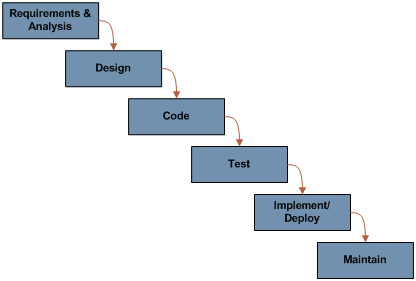
\includegraphics[width=100mm]{images/waterfall.png}
		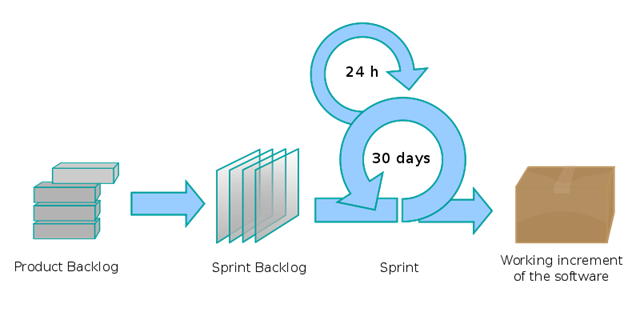
\includegraphics[width=100mm]{images/scrum.png}
		\caption{Software Lifecycles} 
		\label{lifecycles}
	\end{center}
\end{figure}

It has now been shown how to take algorithms, and parallelize them. How does this fit into developing software?
Although software must be built modularly from the beginning, actual parallelization should not occur until the 
end of the software development cycle. This comes from embraced design patterns in software engineering.
If code will take significant refactoring to make parallel, then it is incorrectly written from the beginning.

For example, in the code examples in this report, the function lapply is used. Major sections of code are organized in seperate functions. Changing the function from lapply to parLapply is almost all that is needed
to parallelize the code. 

In Figure \ref{lifecycles}, a few different software lifecycles are listed. \textbf{Waterfall} (top) is a good method if
the requirements for the project never change. Since this is seldom the case in research, Agile 
Development is encouraged. \textbf{Scrum} (bottom) contains many iterations of software development within
the project lifespan, in which a deliverable of the code is delivered. This allows the developers to react to 
changing requirements in the project, as well as a good way to gauge workflow in the project.

This report proposes a hybrid of this, in which there are several different phases of Scrums:

\begin{figure}[h]
	\begin{center}
		\includegraphics[width=160mm]{images/hybrid_scrum.png}
		\caption{Hybrid Scrum Project} 
		\label{hybrid_scrums}
	\end{center}
\end{figure}

The Development scrums start the project. It gives programmers a chance to learn the domain of the project, and try ideas that will be shape the project. This in when profiling of algorithms needs to occur, so reasonable 
data collection results. Implemenation scrums then create the main body of the code. The 
Optimization scrums come next. This is when existing code is streamlined. This phase is important, because it may eliminate the need for complicated parallelization. If granularities, or $P$ values, remain after this 
phase, then the Parallelization can take place.